\section{MOSFET}
\begin{figure}[H]
    \centering
    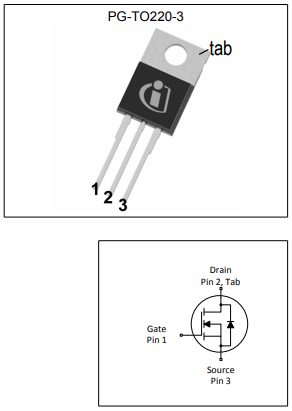
\includegraphics[width=0.5\textwidth]{img/MOSFET/MOSFET.png}
    \caption{IPP015N04NF2S}
    \label{fig:MOSFET:IPP015N04NF2S}
\end{figure}
For MOSFETs, three main factors are crucial: reliability, efficiency, and design. Reliability focuses on the device's limits, which must be prevented during operation. Efficiency refers to how much heat dissipation occurs.
Below, we outline the important aspects for the three main factors when choosing the MOSFET \cite{Proper-Specs-MOSFET}

\subsection{Reliability}
\begin{itemize}
    \item Suffice breakdown voltage protection
    \begin{itemize}
        \item In this case, with a 24 V BLDC motor, a MOSFET with a 40 V breakdown voltage would be sufficient.
    \end{itemize}
\end{itemize}

\subsection{Efficiency}
\begin{itemize}
    \item On-Resistance, $R_{ds(on)}$
    \item Gate charge, $Q_{g}$ 
    \item N-channel 
\end{itemize}

\subsection{Design}
\begin{itemize}
    \item Good thermal flow
    \item EMI
\end{itemize}


An N-channel MOSFET was chosen for implementation in the design. The selected type is the IPP015N04NF2S from Infineon, as shown in Figure \ref{fig:MOSFET:IPP015N04NF2S}. It has the following specifications \cite{Datasheet-MOSFET-IPP015N04NF2S} :
\begin{itemize}
    \item $V_{ds} = 40 V$
    \item $R_{ds(on),\text{max}} = 1.5 m\Omega$
    \item $I_{d} = 193 A$
    \item $Q_{oss} = 117 nC$
    \item $Q_{G}(0V..10V) = 106 nC$
\end{itemize}


